\documentclass{beamer}

% \usetheme{Singapore}
% \usetheme{Malmoe}
\usetheme{Warsaw}

\usepackage[utf8]{inputenc}
\usepackage[russian]{babel}
\usepackage{cmap}
\usepackage{mathrsfs}
\usepackage{changepage}
\usepackage{xcolor}

% \useoutertheme{split}
\useoutertheme{shadow}
\usefonttheme{professionalfonts}
\usepackage{graphicx}
\usepackage{psfrag}
\beamertemplatenavigationsymbolsempty 
\DeclareMathOperator{\sign}{sign}

\setbeamertemplate{footline}[frame number]

\author{Павел Филонов \\ \href{mailto:filonovpv@gmail.com}{filonovpv@gmail.com}}
\title{Введение в машинное обучение}
\subtitle{Метрические методы классификации}

\begin{document}
\begin{frame}[plain]
    \titlepage
\end{frame}
\begin{frame}[plain]{Содержание}
  \tableofcontents
\end{frame}
\section{Гипотезы компактности и непрерывности}
\begin{frame}{Гипотезы компактности и непрерывности}

{\bf Задачи классификации и регресии:}
\begin{itemize}
    \item[] $X$ --- объекты, $Y$ --- ответы;
    \item[] $S = (x_i, y_i)_{i=1}^{\ell}$ --- обучающая выборка.
\end{itemize}

{\bf Гипотеза компактности} (для классификации):
\begin{itemize}
    \item[] {\it Близкие объекты, как правило, лежат в одном классе.}
\end{itemize}

{\bf Гипотеза непрерывности} (для регресии):
\begin{itemize}
    \item[] {\it Близким объектам соответсвуют близкие ответы.}
\end{itemize}

{\bf Формализация понятия <<близости>>:}
\begin{itemize}
    \item[] Задана функция расстояния $\rho : X \times X \rightarrow \left[ 0, \infty \right)$.
\end{itemize}

{\bf Пример.} Евклидово расстояние и его обобщение.
$$
    \rho(x_i, x_k) = \left(\sum\limits_{j=1}^{n}(x_i^j - x_k^j)^2\right)^{1/2},\;  \rho(x_i, x_k) = \left(\sum\limits_{j=1}^{n}w_j(x_i^j - x_k^j)^p\right)^{1/p}
$$
\end{frame}

\begin{frame}{Пример: рост и вес в зависимости от пола}
$N = 200$
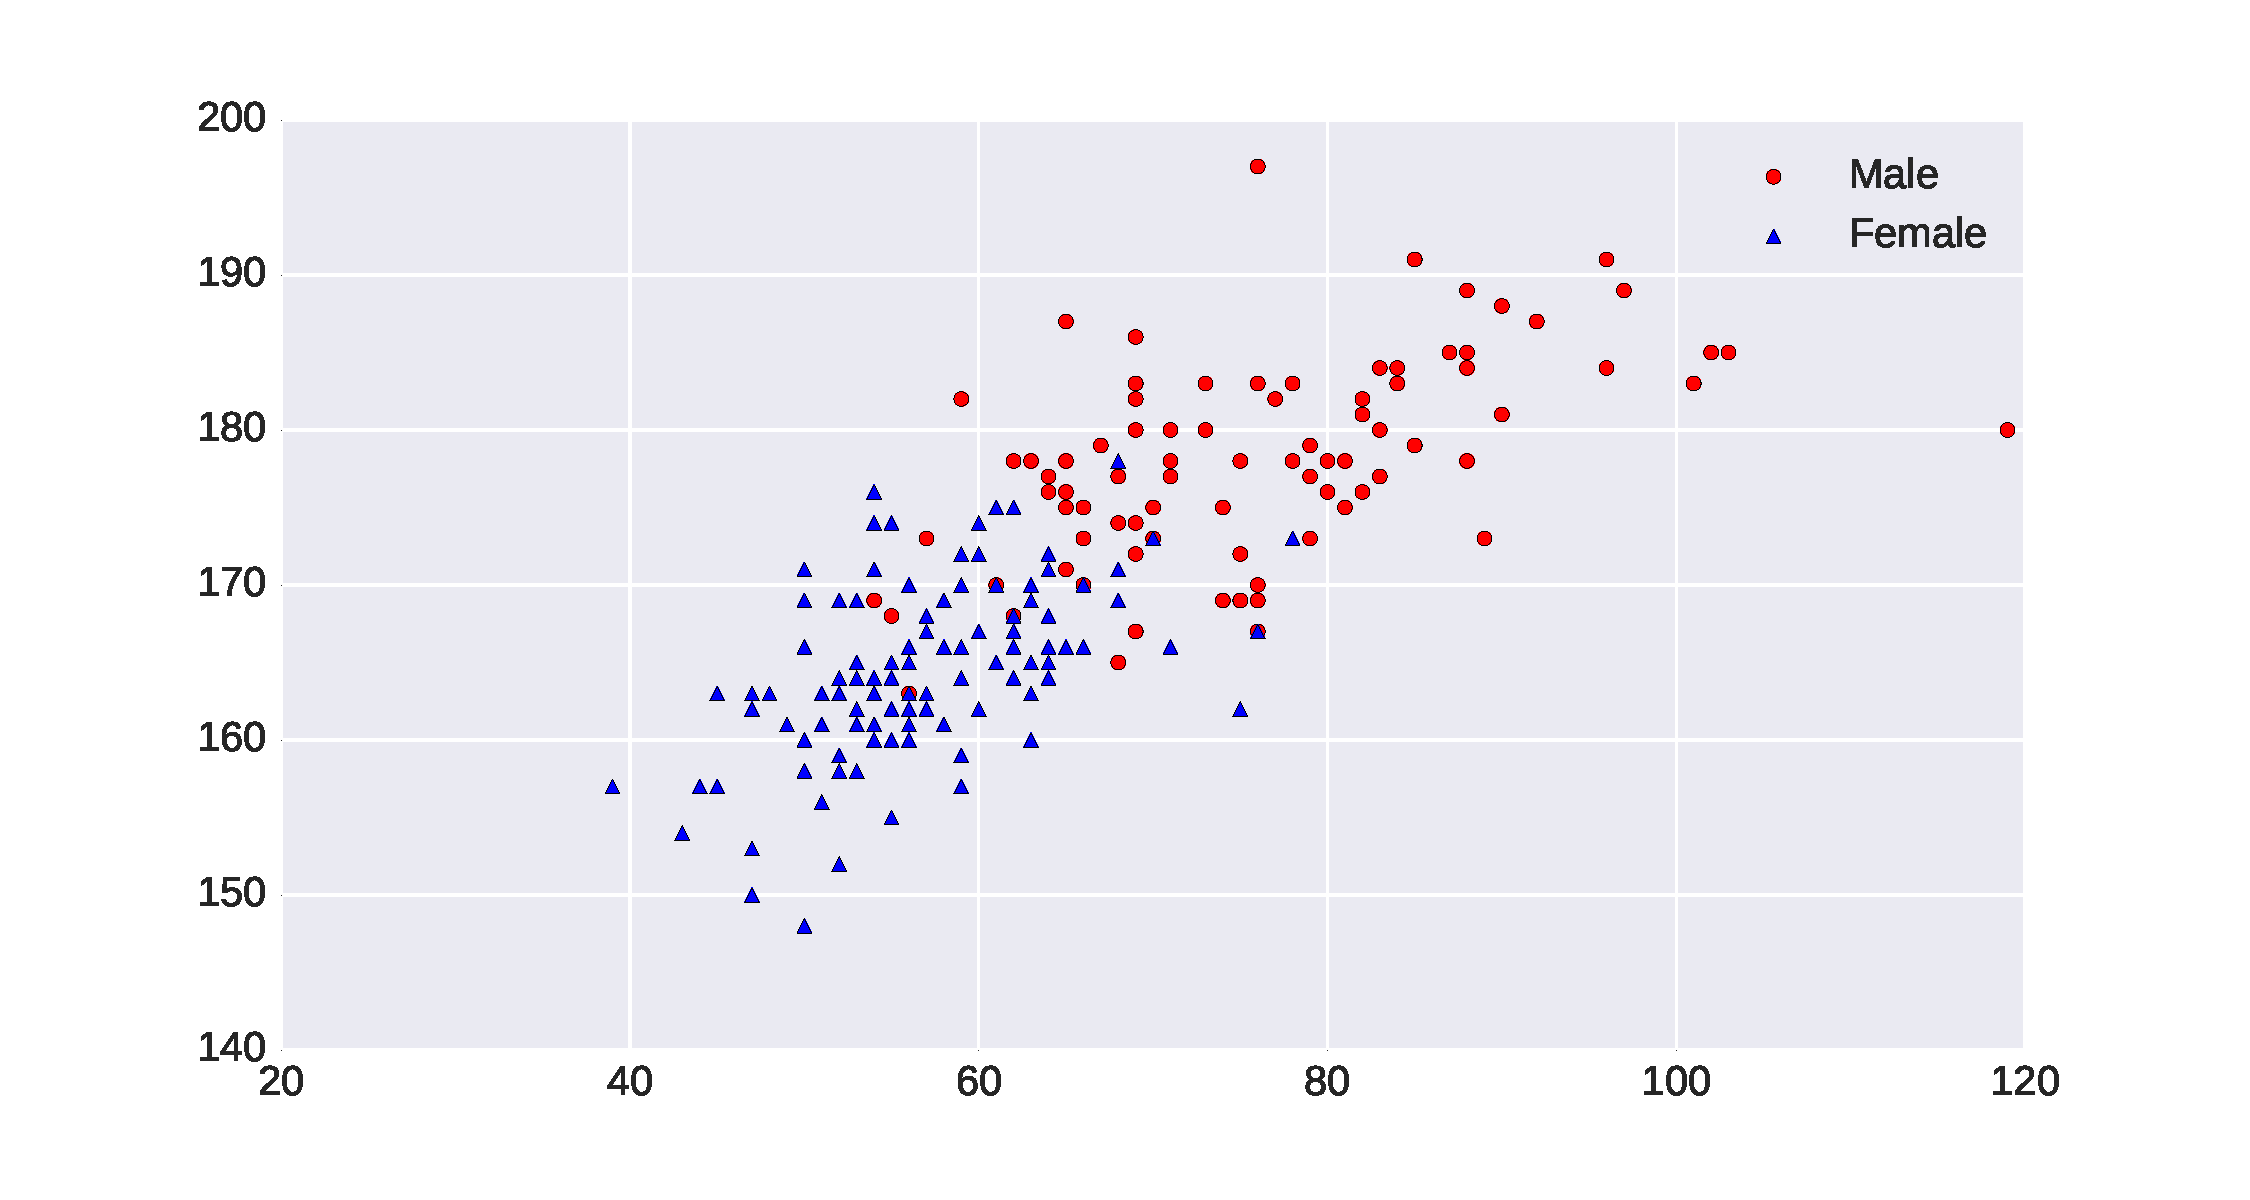
\includegraphics[width=\linewidth]{../fig/height_n_weight.pdf}

\footnotesize
Dataset from \url{https://vincentarelbundock.github.io/Rdatasets/datasets.html}
\end{frame}

%TODO: добавить пример для задачи регрессии

\section{Метрические методы классификации}
\subsection{Обобщённый метрический классификатор}
\begin{frame}{Обобщённый метрический классификатор}
Для произвольного $x \in X$ отранжируем объекты $x_1,\dots,x_\ell$:
$$
    \rho(x, x^{(1)}) \le \rho(x, x^{(2)}) \le \dots \le \rho(x, x^{(\ell)}),
$$
$x^{(i)}$ --- $i$-й сосед объекта $x$ среди $x_1,\dots,x_\ell$;\\
$y^{(i)}$ --- ответ на $i$-м соседе объекта $x$.

{\bf Метричский алгоритм классификации:}
$$
    a(x; S) = \arg\max_{y \in Y}\underbrace{\sum\limits_{i=1}^{\ell}\left[y^{(i)} = y\right]w(i, x)}_{\Gamma_y(x)},
$$
$w(i,x)$ --- вес (степень важности) $i$-го соседа объекта $x$, неотрицателен, не возрастает по $i$.\\
$\Gamma_y(x)$ --- оценка близости объекта $x$ к классу $y$.
\end{frame}

\subsection{Метод ближайших соседей}
\begin{frame}{Метод ближайшего соседа}
$w(i, x) = [i = 1]$.
\vfill
{\bf Преимущества:}
\begin{itemize}
    \item простота реализации;
    \item интерпретируемость решений, вывод на основе прецедентов (case-based reasoning, CBR).
\end{itemize}
{\bf Недостатки:}
\begin{itemize}
    \item неустойчивость к погрешностям (шуму, выбросам);
    \item отсутсвие настраиваемых параметров;
    \item низкое качество классификации;
    \item приходится хранить всю выборку целиком.
\end{itemize}
\end{frame}

\begin{frame}{Метод $k$ ближайших соседей}
$w(i, x) = [i \le k]$.
\vfill
{\bf Преимущества:}
\begin{itemize}
    \item менее чувствителен к шуму;
    \item появился параметр $k$.
\end{itemize}
{\bf Оптимизация числа соседей} $k$:
функционал скользящего контроля leave-one-out
$$
LOO(k, S) = \sum\limits_{i=1}^{\ell}\left[a(x_i; S\setminus\{x_i\}; k) \ne y_i\right] \rightarrow \min_k.
$$
{\bf Проблема:}
\begin{itemize}
    \item неоднозначность классификации при $\Gamma_y(x) = \Gamma_s(x),\; y \ne s$.
\end{itemize}
\end{frame}

\begin{frame}{Пример. Зависимость LOO от числа соседей}
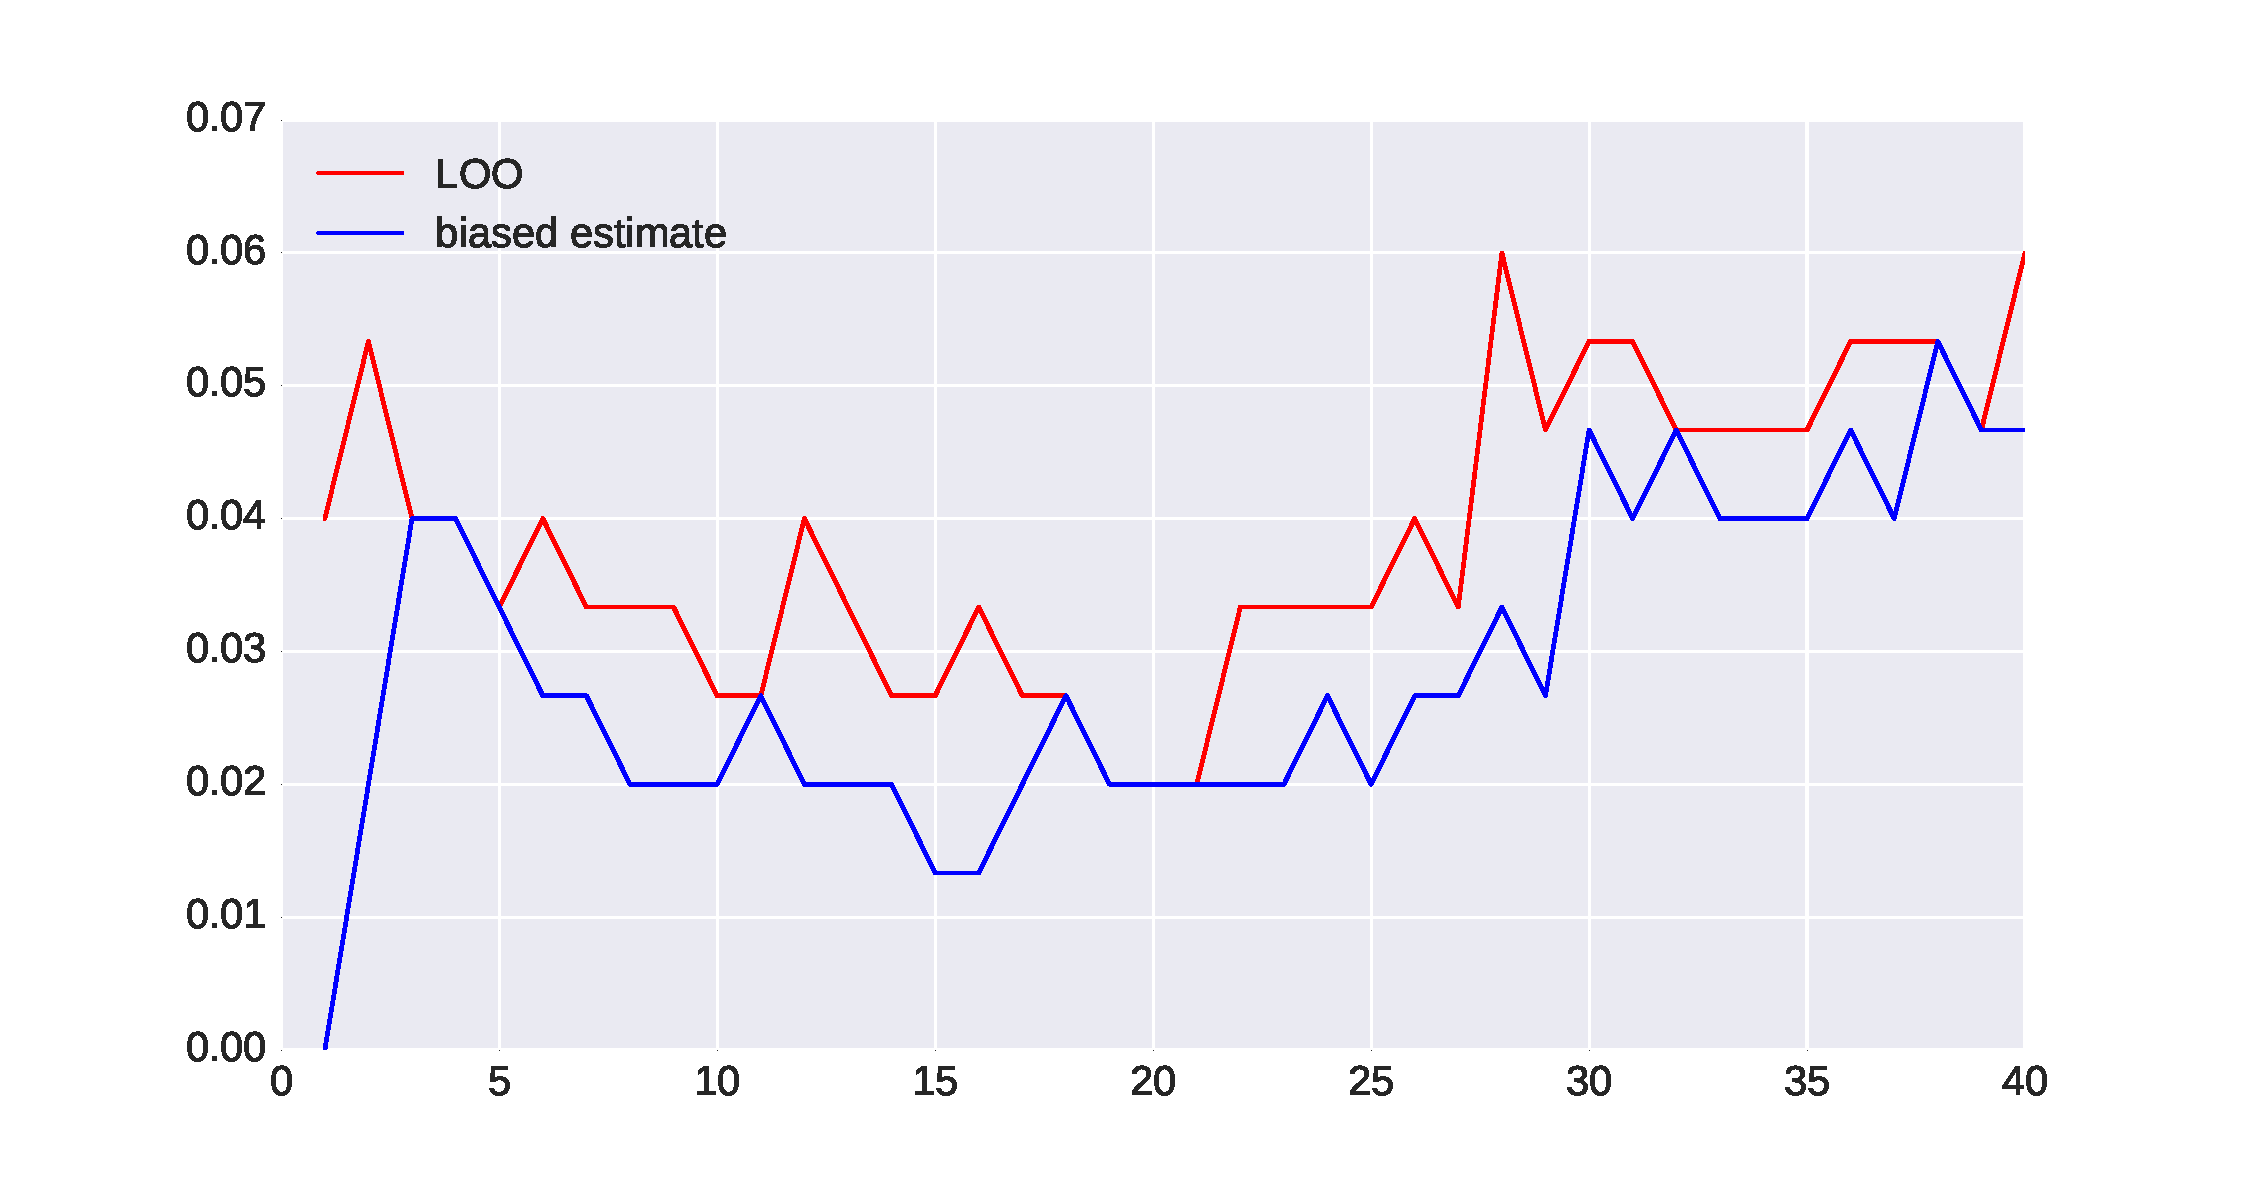
\includegraphics[width=\linewidth]{../fig/iris_knn_loo.pdf}
\begin{itemize}
    \item \textcolor{red}{несмещенная доля ошибок LOO}
    \item \textcolor{blue}{смещенная доля ошибок, когда объект учитывается как сосед самого себя}
\end{itemize}
\end{frame}

\begin{frame}{Метод $k$ взвешенных ближайших соседей}
$w(i,x) = [i \le k] w_i,$\\
где $w_i$ --- вес, зависящий только от номера соседа;

{\bf Возможные эвристики:}
\begin{itemize}
    \item $w_i = \frac{k+1-i}{k}$ --- линейно убываюшие веса;
    \item $w_i = q^i$ --- экспоненциально убывающие веса, $0 < q < 1$.
\end{itemize}
{\bf Проблемы:}
\begin{itemize}
    \item как более обоснованно задавать веса?
    \item возможно, было бы лучше, если бы вес $w(i,x)$ зависел не от порядкового номера соседа $i$, а от расстояния до него $\rho(x, x^{(i)})$.
\end{itemize}
\end{frame}

\subsection{Окно Парзена и потенциальные функции}
\begin{frame}{Метод окна Парзена}
$w(i,x) = K(\frac{\rho(x, x^{(i)})}{h})$, где $h$ --- ширина окна, \\
$K(r)$ --- ядро, не возрастает и положительно на $[0,1]$.

{\bf Метод парзеновского окна фиксированной ширины:}
$$
a(x; S, h, K) = \arg\max_{y \in Y}\sum\limits_{i=1}^{\ell}[y_i = y]K(\frac{\rho(x, x_i)}{\color{red} h}).
$$
{\bf Метод парзеновского окна переменной ширины:}
$$
a(x; S, k, K) = \arg\max_{y \in Y}\sum\limits_{i=1}^{\ell}[y_i = y]K(\frac{\rho(x, x_i)}{\color{red}\rho(x, x^{(k+1)})}).
$$

{\bf Оптимизация параметров} --- по критерию LOO:
\begin{itemize}
    \item выбор ширины окна $h$ или числа соседей $k$;
    \item выбор ядра $K$.
\end{itemize}
\end{frame}

\begin{frame}{Парзеновское окно фиксированной ширины $h$}

{\bf Пример:} двумерная выборка, два класса $Y = \{-1, +1\}$.
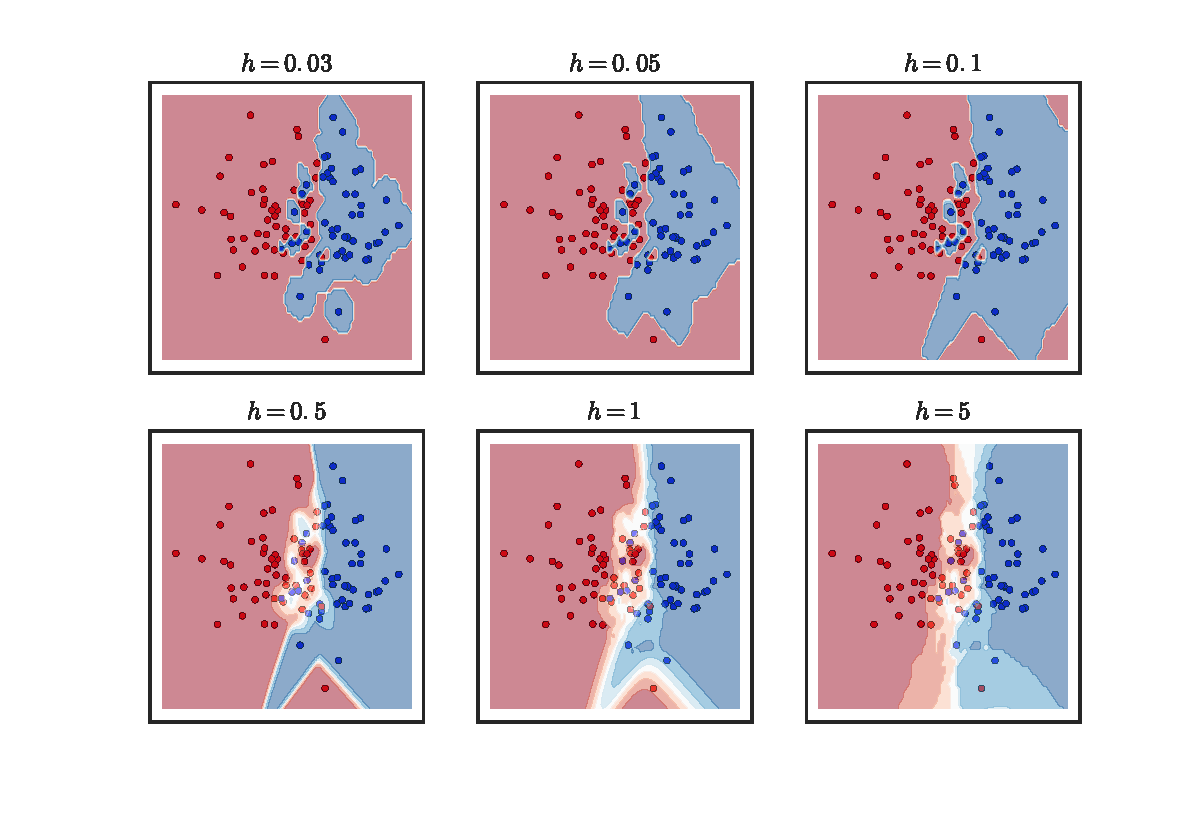
\includegraphics[width=\linewidth]{../fig/knn.pdf}
\end{frame}

\begin{frame}{Часто используемые ядра}
\begin{center}
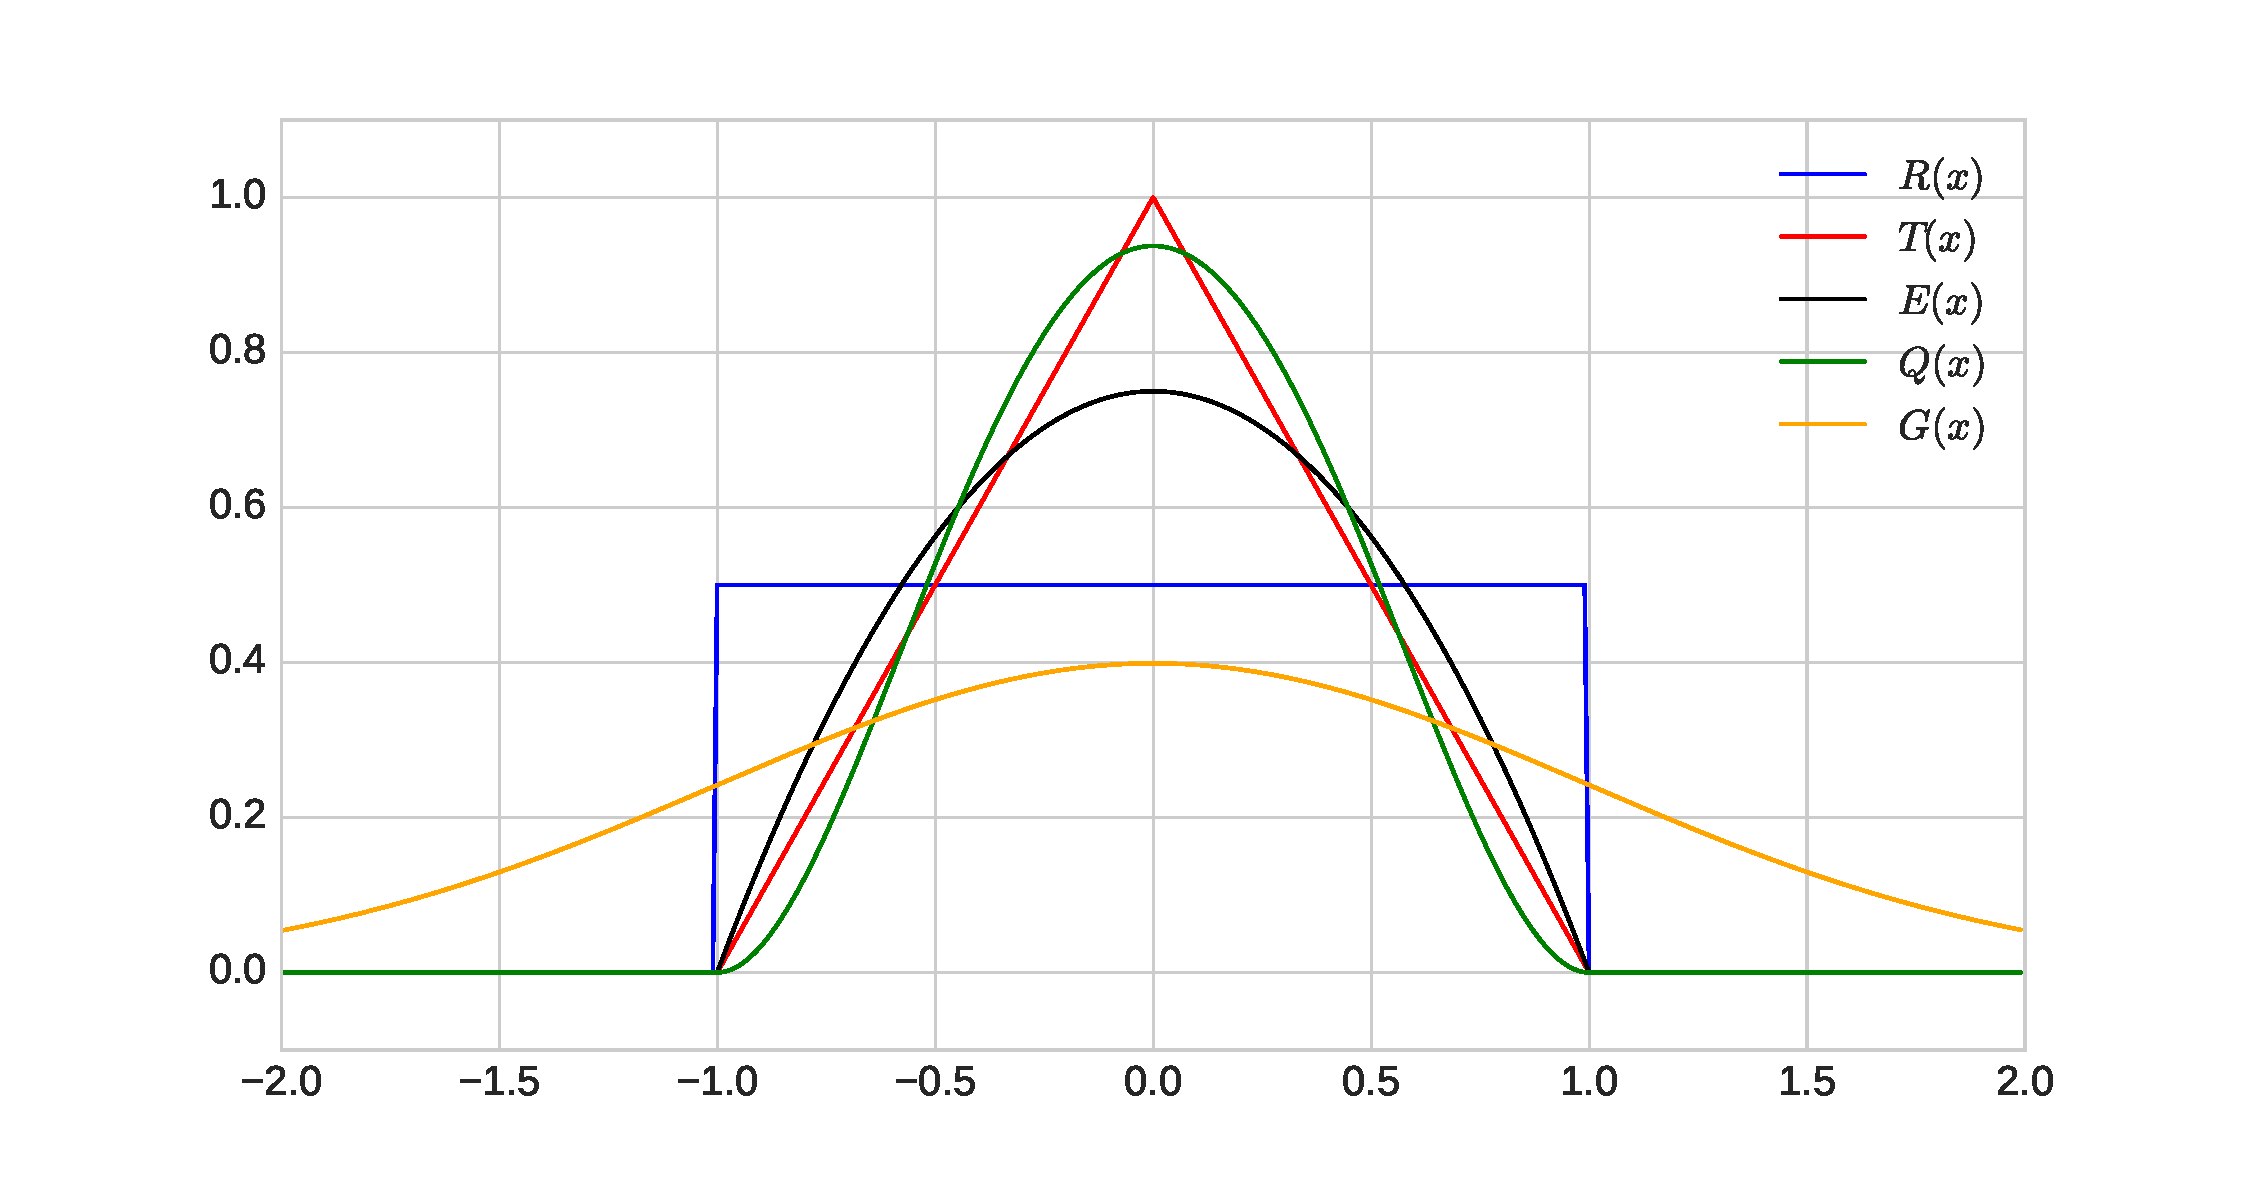
\includegraphics[width=0.8\textwidth]{../fig/cores.pdf}
\end{center}
\begin{itemize}
    \item[] $R(x) = 0.5[|x| \ge 1]$ --- прямоугольное;
    \item[] $T(x) = (1 - |x|)[|x| \ge 1]$ --- треугольное;
    \item[] $E(x) = 0.75(1-x^2)[|x| \ge 1]$ --- ядра Епанечникова;
    \item[] $Q(x) = 15/16(1-x^2)^2[|x| \ge 1]$ --- квадратичное;
    \item[] $G(x) = \frac{1}{\sqrt{2\pi}}\exp\left(-x^2/2\right)$ --- ядро Гаусса.
\end{itemize}
\end{frame}
\begin{frame}{Метод потенциальных функций}
$w(i, x) = \gamma^{(i)}K\left(\frac{\rho(x,x^{(i)})}{h^{(i)}}\right)$

Более простая записть (можно не ранжировать объекты)
$$
a(x; S) = \arg\max_{y \in Y}\sum\limits_{i=1}^{\ell}[y_i=y]\gamma_iK\left(\frac{\rho(x, x_i)}{h_i}\right),
$$
где $\gamma_i$ --- веса объектов, $\gamma_i \ge 0,\;h_i>0$.

{\bf Физическая аналогия:}
\begin{itemize}
    \item[] $\gamma_i$ --- величина <<заряда>> в точке $x_i$;
    \item[] $h_i$ --- <<радиус действия>> потенциала с центром в точке $x_i$;
    \item[] $y_i$ --- знак <<заряда>> (в случае двух классов $Y = \{-1, +1\}$);
\end{itemize}
\end{frame}

\begin{frame}{Резюме}
    \begin{itemize}
        \item метрические классификаторы --- одни из самых простых;
        \item качество классификации определяется качеством метрики;
        \item что можно обучать:
        \begin{itemize}
            \item число ближайших соседей $k$;
            \item ширину окна $h$;
            \item веса объектов;
            \item метрику;
            \item веса признаков в метрике;
            \item функцию ядра $K(r)$.
        \end{itemize}
    \end{itemize}
\end{frame}
\end{document}